\documentclass[11pt]{article}
\usepackage[margin=1.0in]{geometry}
\usepackage{amsmath}
\usepackage{url,  multirow}
\usepackage{booktabs}
\usepackage{longtable}
\usepackage{algorithm}
\usepackage{graphicx} 

\usepackage[authoryear,round]{natbib}

\newcommand{\eps}{\epsilon}
\newcommand{\veps}{\varepsilon}


\title{\textbf{Appendix 1:} Management Procedures}
\author{}
%\date{\today}

\begin{document}

\maketitle

\tableofcontents
\newpage\clearpage

\section{Management Procedures}

\subsection{Empirical}
 
\subsubsection{CCSBT}
CCSBT developed an MP where The TAC is an average of candidate TACs obtained from two HCRs \citep{hillary2013sbthcr}.

The first HCR used a single index for the adult stock and then increased or decreased the current catch if that index was increasing or decreasing respectively, while the second compared the current value of an index to a reference period.

In the first, the TAC is updated depending on the trend in an index ($I$)

\begin{equation}
 TAC^1_{y+1}=TAC_y\times \left\{\begin{array}{rcl}  {1-k_1|\lambda|^{\gamma}} & \mbox{for} & \lambda<0\\[0.35cm]
{1+k_2\lambda} & \mbox{for} & \lambda\geq 0 
    \end{array}\right.
\end{equation}
        

where $\lambda$ is the slope in the regression of $\ln I_y$ against year for the most recent $n$ years. $k_1$ and $k_2$ are \textit{gain} parameters and $\gamma$ actions asymmetry so that decreases in the index do not result in the same relative change as as an increase.

%giving 4 tunable parameters (\textbf{Table} \ref{tab1})

The second HCR uses both an adult and juvenile indies i.e.

\begin{equation} 
 %\begin{align*}
     TAC^2_{y+1} = 0.5\times\left(TAC_y+C^{\rm targ}_y\Delta^R_y\right)\\
 %\end{align*}
\end{equation}

where 

\begin{equation} 
 %\begin{align*}
  C^{\rm targ}_y = 
  \left\{\begin{array}{rcl} {\delta \left[\frac{I_{y}}{I^*}\right]^{1-\veps_b}} & \mbox{for} & I_{y}\geq I^*\\
                            {\delta \left[\frac{I_{y}}{I^*}\right]^{1+\veps_b}} & \mbox{for} & I_{y}<I^* \\
    \end{array}\right.
 %\end{align*}
\end{equation}

\begin{equation} 
\Delta^R_y = \left\{\begin{array}{rcl}{\left[\frac{\bar{R}}{\mathcal{R}}\right]^{1-\veps_r}} & \mbox{for} & \bar{R}\geq\mathcal{R}\\[0.35cm]
{\left[\frac{\bar{R}}{\mathcal{R}}\right]^{1+\veps_r}} & \mbox{for} & \bar{R}<\mathcal{R}
\end{array}\right.
\end{equation}


where $\delta$ is the \textit{target} catch; $I^*$ the \textit{target} adult index (e.g. a mean observed CPUE corresponding to a period where the stock was at a desired fraction of $B_0$ or $M_{MSY}$) and 
$\bar{R}$ is the average recent juvenile biomass i.e.

\begin{equation}
    \bar{R}=\frac{1}{\tau_R}\sum\limits_{i=y-\tau_R+1}^{y}R_i
 \end{equation}

 
$\mathcal{R}$ is a ``limit'' level derived from the mean recruitment over a reference period; while $\veps[0,1]$ actions asymmetry so that increases in TAC do not occur at the same level as decreases.

%There are therefore 5 tunable parameters, \textbf{Table} \ref{tab2}

 
\begin{table}[h]
\centering
\caption{Derivative MP tunable parameters}
\begin{tabular}{p{3cm}p{1.2cm}p{6cm}p{2cm}} 
  \hline
  Parameter & Symbol & Description & Default \\ 
  \hline
   Gain term &$b$      & Sets change based on adult index in HCR 1         & 0.25\\
   Gain term &$r$      & Sets sets change based on recruit index HCR 1     & 0.75\\
   Gain term &$k_1$    & Sets decrease level when stock declines in HCR 2  &1.5 \\
   Gain term &$k_2$    & Sets increase level when stock increases in HCR 2 &3.0 \\
   Exponent  &$\gamma$ & Additional decrease control in HCR 2              & 1  \\
  \hline
\end{tabular}
\end{table}



\newpage\clearpage
\subsubsection{Proportional}
A proportional control rule (P) is so called as the action is determined in proportion to the error between a signal and a reference value

\begin{equation} 
 %\begin{align*}
  C^{\rm targ}_y = 
  \left\{\begin{array}{rcl} 
      {\delta \left[\frac{I_{y}}{I^*}\right]^{1-\veps_k1}} & \mbox{for} & I_{y}\geq I^*\\
      {\delta \left[\frac{I_{y}}{I^*}\right]^{1+\veps_k2}} & \mbox{for} & I_{y}<I^* \\
        \end{array}
  \right.
 %\end{align*}
\end{equation}

where $\delta$ is the target catch and $k_1$ and $k_2$ are the gain terms 

The TAC is then the average of the last TAC and the value output by the HCR. 

\begin{equation} 
     TAC_{y+1} = 0.5\times\left(TAC_y+C^{\rm targ}_y\right)\\
\end{equation}

\begin{table}[h]
\centering
\caption{Proportion MP tunable parameters}
\begin{tabular}{p{3cm}p{1.2cm}p{6cm}p{2cm}} 
  \hline
  Parameter & Symbol & Description & Default \\ 
  \hline
  Gain term & $k_1$ & Sets decrease level when stock declines  & 0.25\\
  Gain term & $k_2$ & Sets increase level when stock increases   & 0.75\\
  \hline
\end{tabular}
\end{table}


\newpage\clearpage
\subsubsection{Derivative}
A derivative control rule (D) is so called as the control signal is derived from the trend in the signal, i.e. to the derivative of the error. 


\begin{equation}
 TAC^1_{y+1}=TAC_y\times 
 \left\{\begin{array}{rcl}  
    {1-k_1|\lambda|^{\gamma}} & \mbox{for} & \lambda<0\\[0.35cm]
    {1+k_2\lambda} & \mbox{for} & \lambda\geq 0 
 \end{array}\right.
\end{equation}

where $\lambda$ is the slope in the regression of $\ln I_y$ against year for the most recent $n$ years and $k_1$ and $k_2$ are \textit{gain} parameters and $\gamma$ actions asymmetry so that decreases in the index do not result in the same relative change as as an increase.

The TAC is then the average of the last TAC and the value output by the HCR. 

\begin{equation} 
     TAC_{y+1} = 0.5\times\left(TAC_y+C^{\rm targ}_y\right)\\
\end{equation}



\begin{table}[h]
\centering
\caption{Derivative MP tunable parameters}
\begin{tabular}{p{3cm}p{1.2cm}p{6cm}p{2cm}} 
  \hline
  Parameter & Symbol & Description & Default \\ 
  \hline
   Gain term &$k_1$    & Sets decrease level when stock declines  &1.5 \\
   Gain term &$k_2$    & Sets increase level when stock increases &3.0 \\
   Exponent  &$\gamma$ & Additional decrease control              & 1  \\
  \hline
\end{tabular}
\end{table}




\newpage\clearpage
\subsubsection{iRate}
The iRate Management Procedure uses CPUE as an index of biomass (I) and sets a total allowable catch or TAC ($\bar{S}$) that, over most of the range of CPUE, is proportional to that index.

In each year a smoothed index ($\bar{I}$) is calculated using an exponential moving average with the responsivesness control parameter, $r$:

\begin{equation}
\bar{I_t}=rI_t+(1-r)\bar{I}_{t+1}
\end{equation}


Higher values of $r$ produce greater responsiveness because they put more weight on more recent values of CPUE and produce a index that is less smoothed. When $r = 1$ there is no smoothing and $\bar{I_t}=r\bar{I_t}$.
Smoothing may be advantageous in that it reduces the influence of annual random variation in CPUE due catchability or operational variations. However, smoothing also reduces adds a lag to the index.

Using $\bar{I}$ the recommended catch scaler ($\bar{S}$) is calculated as follows	. 

 
\begin{equation}
\bar{S} = \left\{ \begin{array}{ll}
	0                   			  &\mbox{$\bar{I} < i_t$} \\
	m\hat{S}            			  &\mbox{$\bar{I} > i_t$} \\
	\frac{m\hat{S}}{i_t-i_l}(\bar{I}-i_l)     &\mbox{otherwise}\\
		  \end{array}
	  \right.
\end{equation}


The recommended catch scaler is used to calculate the recommended TAC ($\bar{S}$) by multiplying the harvest rate by the biomass index,

\begin{equation}
\bar{C}=min(\bar{S}\bar{I},u)
\end{equation}

which is applied to the fishery in the following year,

\begin{equation}
C_{t+1} = \bar{C}_\phi
\end{equation}

where $\phi$ is a lognormally distributed multiplicative error with mean of 1 and standard deviation of $\veps$,

\begin{equation}
\phi \sim LN(1,\veps)
\end{equation}

\begin{table}[h]
\centering
\caption{iRate tunable parameters}
\begin{tabular}{p{3cm}p{1.2cm}p{6cm}p{2cm}} 
  \hline
  Parameter & Symbol & Description & Default \\ 
  \hline
  Reference years   &$r$&    Years used when computing reference values            & 0.5 \\
  Responsiveness    &$m$&    Target harvest rate relative to historic levels     
  Target harvest             i.e 0.9 = 90\% of historic average                    & 0.9 \\
  Threshold index   &$i_t$&  Index at which the harvest rate is reduced 
                             relative to historic levels i.e. 0.7 = 
                             reduce harvest rate when the biomas index is
                             at 70\% of historic levels                            & 0.7 \\ 
  Limit index       &$i_l$&  Index at which harvest rate is zero
			     relative to historic levels i.e. 0.2 = close the
			     fishery when the biomas index is at 20% of
			     historic levels                                       & 0.2 \\ 
  Maximum change    &$f$&    Maximum allowable percenatge change in
                             effort                                                & 0.4 \\ 
  Maximum TAC       &$u$&    Maximum total allowable catch                         & 1000\\ 
  \hline
\end{tabular}
\end{table}



\newpage\clearpage
\subsection{Model Based}

\subsubsection{MPB}
In a model based MP a stock assessment model is used to derive stock status relative to limit and target reference points and based on this to set a TAC. 

A limit requires something to be done before it is reached and a target is a reward for doing something good. The standard fisheries HCR is a hockey stick (\textbf{Figure} \ref{fig:hcr}) where for any biomass a corresponding fishing mortality is given, which is then used to derive a TAC. The hockey stick is defined by two points, the target fishing mortality ($F_{target}$) and a threshold ($B_{threshold}$)  that cause management action to be triggered if it is breached. Above $B_{threshold}$ $F_{target}$ defines a target level of fishing mortality that management seeks to achieve, below  $B_{threshold}$ F declines linearly to the limit biomass ($B_{lim}$).


\begin{figure*}[htbp]
\centering
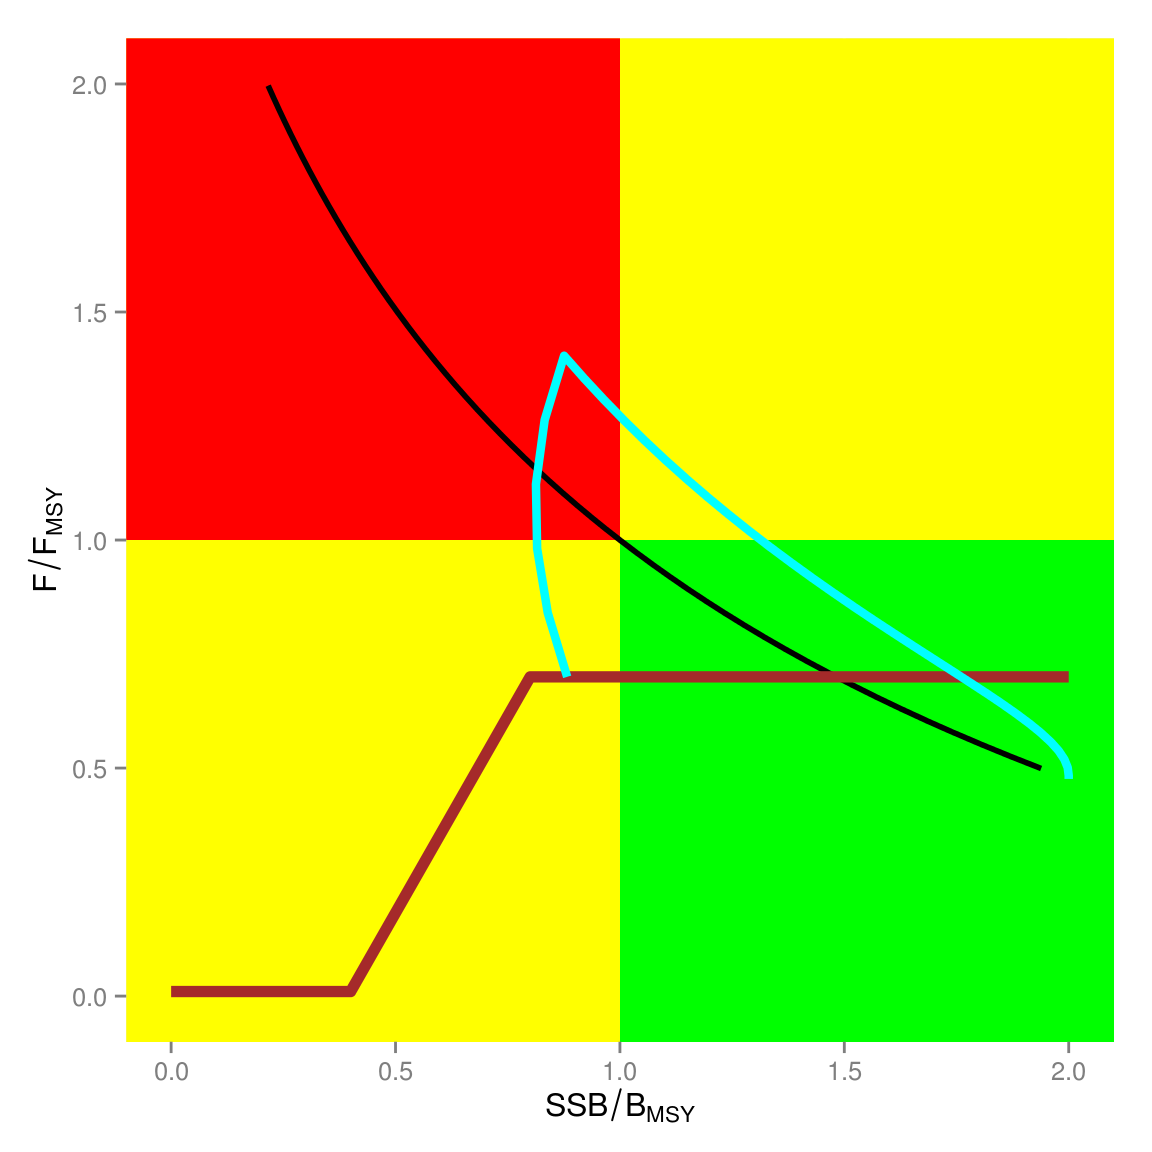
\includegraphics[width=6in]{../png/hcr.png}
\label{fig:hcr}
\caption{Harvest Control Rule (brown) plotted on a phase plot of harvest rate relative to $F_{MSY}$ and stock biomass relative to $B_{MSY}$;
the light line is the simulated stock and the black line is the replacement line.}
\end{figure*}


Setting targets and limits requires deciding upon the values used to define these two points. For example using a stock assessment there are severall potential reference points such as those based on maximum sustainable yield ($MSY$), i.e. the biomass at which this is achived ($B_{MSY}$ and the fishing mortlaity ($F_{MSY}$) that will achieve it.

The biomass of a stock next year ($B_{t+1}$) is equal to the biomass this year $B_{t}$, less the catch ($C_t$) plus the surplus production ($P_t$) i.e. 

\begin{equation}  B_{t+1}=B_{t}-C_{t}+P_{t}\end{equation}  

$P$ is given by the Pella-Tomlinson surplus production function \citep{pella1969generalized}

\begin{equation}\frac{r}{p}\cdot~B(1-(\frac{B}{K})^p)\end{equation}  




\newpage\clearpage\clearpage
\bibliography{refs.bib} 
\bibliographystyle{abbrvnat} 

\end{document}
